% Cinq molécules à nommer (exercice 2, chapitre 11)
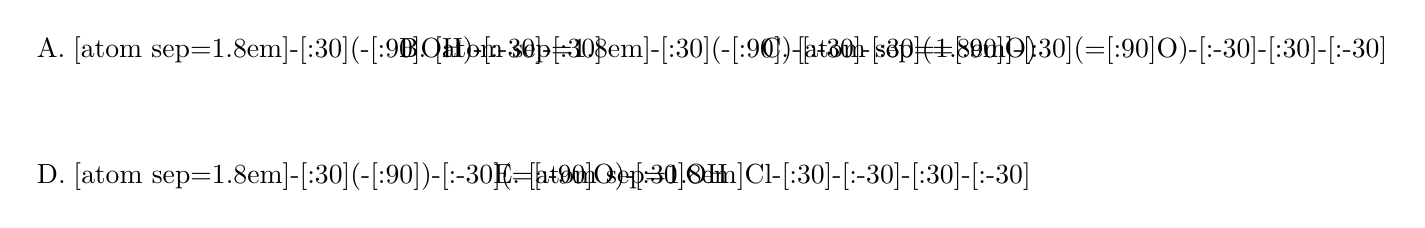
\begin{tikzpicture}[x=1cm,y=1cm]
\node[anchor=west] at (0,2.1) {\otLabel{A.}\;\chemfig[atom sep=1.8em]{-[:30](-[:90]OH)-[:-30]-[:30]}};
\node[anchor=west] at (4.6,2.1) {\otLabel{B.}\;\chemfig[atom sep=1.8em]{-[:30](-[:90])-[:-30]-[:30](=[:90]O)}};
\node[anchor=west] at (9.2,2.1) {\otLabel{C.}\;\chemfig[atom sep=1.8em]{-[:30](=[:90]O)-[:-30]-[:30]-[:-30]}};
\node[anchor=west] at (0,0.5) {\otLabel{D.}\;\chemfig[atom sep=1.8em]{-[:30](-[:90])-[:-30](=[:-90]O)-[:30]OH}};
\node[anchor=west] at (5.8,0.5) {\otLabel{E.}\;\chemfig[atom sep=1.8em]{Cl-[:30]-[:-30]-[:30]-[:-30]}};
\end{tikzpicture}
\par\smallskip\legende{Les formules topologiques de cinq molécules organiques. Dans la molécule B, le carbone du groupe C=O porte aussi un atome d'hydrogène.}
